\documentclass{amsart}

\include{RDTP-Preamble}

\begin{document}

\title{The balanced tensor product of module categories}

\begin{abstract}
A key role in the theory of tensor categories is played by the relative Deligne tensor product $\cM \boxtimes_\cC \cN$ which is a higher dimensional analogue of the tensor product of a right and a left module over a non-commutative ring.  The relative Deligne tensor product is characterized by a universal property, but such a characterization does not guarantee existence.  In this paper, we give a construction of the relative Deligne tensor product for finite tensor categories (in the sense of Etingof-Ostrik) and their finite module categories.  This generalizes results of Etingof-Nikshych-Ostrik in the semisimple case.  Explicitly, we realize the relative Deligne tensor product over $\cC$ as a category of bimodule objects in $\cC$.
\end{abstract}

\author{Christopher L. Douglas}
\address{Mathematical Institute\\ University of Oxford\\ Oxford OX1 3LB\\ United Kingdom}
\email{cdouglas@maths.ox.ac.uk}
\urladdr{http://people.maths.ox.ac.uk/cdouglas}
      	
\author{Christopher Schommer-Pries}
\address{Department of Mathematics\\ Max Planck Institute for Mathematics \\ 53111 Bonn \\ Germany}
\email{schommerpries.chris.math@gmail.com}
\urladdr{http://sites.google.com/site/chrisschommerpriesmath}

\author{Noah Snyder}
\address{Department of Mathematics\\ Indiana University\\ Bloomington, IN 47401\\ USA}
\email{nsnyder@math.columbia.edu}
\urladdr{http://www.math.columbia.edu/\!\raisebox{-1mm}{~}nsnyder/}

\thanks{CD was partially supported by a Miller Research Fellowship, CSP was partially supported by NSF fellowship DMS-0902808 and the Max Planck Institute for Mathematics,  NS was partially supported by NSF fellowship DMS-0902981 and DARPA HR0011-11-1-0001.
}


\maketitle	

\tikzexternaldisable

\setcounter{tocdepth}{2}
\tableofcontents



\section{Introduction}

Tensor categories are a higher dimensional analogue of algebras.  Just as modules and bimodules play a key role in the theory of algebras, the analogous notions of module categories and bimodule categories play a key role in the study of tensor categories (as pioneered by Ostrik \cite{MR1976459}).  One of the key constructions in the theory of modules and bimodules is the relative tensor product $M \otimes_A N$ which is universal for $A$-balanced bilinear functions out of $M \times N$.   A similar role is played by the balanced tensor product of module categories $\cM \boxtimes_\cC \cN$ in the theory of tensor categories (for example, see \cite{MR1966524, 0909.3140, MR2511638, MR2909758, 1202.4396, MR3022755, MR3063919}).  This balanced tensor product is called the relative Deligne tensor product, and it is universal for certain balanced functors.  Since it is defined by a universal property, if it exists this tensor product is unique up to unique isomorphism.  However, in order to prove existence one needs a direct construction.  Such a construction depends on $\cM$, $\cC$, and $\cN$ satisfying certain niceness properties.  

The relative Deligne tensor product was first constructed by Etingof-Nikshych-Ostrik under the assumption that $\cC$ is a fusion category and $\cM$ and $\cN$ are finite semisimple module categories \cite{0909.3140}.  A construction of the relative Deligne tensor product for certain non-semisimple categories can also be extracted from \cite[Thm 3.1]{1102.3411}.   In this paper, we give a construction of the Deligne tensor product under the assumption that $\cC$ is a finite tensor category in the sense of \cite{EO-ftc} and $\cM$ and $\cN$ are finite module categories.  

\begin{theorem}
If $\cC$ is a finite tensor category, $\cM$ is a finite right $\cC$-module category, and $\cN$ is a finite left $\cC$-module category, then there exists a finite tensor category $\cM \boxtimes_\cC \cN$ representing $\cC$ balanced right exact bilinear functors out of $\cM \times \cN$.
\end{theorem}

The key result underlying our construction shows that any module category can be realized as a category of modules.  It is due to Ostrik in the fusion case, Etingof-Ostrik for exact module categories, and in the general case appears in Etingof-Gelaki-Nikshych-Ostrik's lecture notes.

\begin{theorem}{\cite[Thm 2.11.6]{EGNO}, \cite[\S 3.2]{EO-ftc}, \cite[Thm 1]{MR1976459}} %\label{thm:EGNO2.11.6}
	\CSP{I commented out the label to this theorem as it was multiply defined.}
	If $\cM$ is a finite left module category over a finite tensor category $\cC$, then there exists an algebra object $A \in \cC$ together with an equivalence of left $\cC$-module categories between $\cM$ and the category of right $A$-module objects in $\cC$.  Similarly, any finite right module category over a finite tensor category is equivalent to a category of left $A$-modules for some algebra object $A \in \cC$.
\end{theorem}

Using this theorem we have the following explicit construction of the relative Deligne tensor product.

\begin{theorem}
If $\cC$ is a finite tensor category and $A, B \in \cC$ are algebra objects, then the category of $A\text{-Mod-}B$ objects in $\cC$ together with the obvious forgetful functors satisfies the universal property of the relative Deligne tensor product $(A\text{-Mod}) \boxtimes_\cC (\text{Mod-}B)$.
\end{theorem}

The balanced tensor product will play a key role in our study of the $3$-category of finite tensor categories and the associated local toplogical field theories in our papers \cite{3TC, DTCI}.  One of our goals in writing this paper is that it can serve as a self-contained introduction to the parts of EGNO's theory which are needed in those papers.  In order to keep this paper self-contained, and to clarify several details of where the assumptions of finiteness and rigidity come into the argument, we have reproved a few results from Etingof, Gelaki, Nikshych, and Ostrik's work and given the proofs of a few results that they left as exercises to the reader.

\section{Linear categories and tensor categories} \label{sec:tc-lincat}

\subsection{Finite linear categories}

	Let $k$ be a fixed ground field, let $\overline{\Vect}_k$ be the category of (possibly infinite-dimensional) $k$-vector spaces, and let $\Vect_k$ be the category of finite-dimensional $k$-vector spaces.   A {\em linear category} is an abelian category with a compatible enrichment over $\overline{\Vect}_k$. \CD{What does compatible mean here that isn't in the definition of enrichment?} \CSP{This means that the additive structure on homs from the abelian category agrees with the additive structure from the Vect-enrichement.}
A {\em linear functor} is an additive functor, that is also a functor of $\overline{\Vect}_k$-enriched categories. 

\begin{warning}
	In \cite{3TC, DTCI} we will use the word ``linear functor" to mean what we call ``right exact linear functor" in this paper.  This is because in the $3$-category of finite tensor categories the $3$-morphisms are assumed to be right exact, because the Deligne tensor product of linear categories is only functorial with respect to right exact functors.  Since this paper concerns the definition of the Deligne tensor product itself, we will not use this convention here.
\end{warning}

Recall the following standard terminology:
\begin{itemize}
	\item[-] A object of a linear category is {\em simple} if it admits no non-trivial subobjects. The endormorphism ring of any simple object is a division algebra over $k$. 
	\item[-] An object $X$ of a linear category has {\em finite length} if every strictly decreasing chain of subobjects $X = X_0 \supsetneq X_1 \supsetneq X_2 \supsetneq  \cdots$ has finite length. 
	\item[-] A linear category is {\em semisimple} if every object splits as a direct sum of simple objects, or equivalently, if every short exact sequence splits. If in addition every object has finite length, then every object splits as a {\em finite} direct sum of simple objects.
	\CD{what?} %finite?
	\CSP{Is this better?}
	\item[-] A linear category {\em has enough projectives} if for every object $X$, there is a project object $P$ with a surjection $P \twoheadrightarrow X$. 
\end{itemize}


\begin{definition} % This is from EGNO Definition 1.18.2.
	A linear category $\cC$ is {\em finite} if 
	\begin{enumerate}
		\item[1.] $\cC$ has finite-dimensional spaces of morphisms;
		\item[2.] every object of $\cC$ has finite length;
		\item[3.] $\cC$ has enough projectives%, i.e. every simple object of $\cC$ has a projective cover
		; and
		\item[4.] there are finitely many isomorphism classes of simple objects.  
	\end{enumerate}
\end{definition}

The following proposition is well-known, and justifies the definition of finiteness.

\begin{proposition}
A linear category is finite if and only if it is equivalent to the category $\Mod{A}{}$ of finite-dimensional modules over a finite-dimensional $k$-algebra $A$.
\end{proposition}
\begin{proof}
	It is standard that, for $A$ a finite-dimensional $k$-algebra, the linear category $\Mod{A}{}$ satisfies the four conditions. \NS{Should we say more about this first sentence?  Isn't this whole proposition standard?  Should we add a citation?}
	% The only property which is not immediate is that every module admits a {\em projective cover}, that is an epimorphism onto that module whose source is projective and whose kernel is superfluous. However this is precisely the classical fact that every finite-dimensional algebra over a field is semiperfect.
	Now assume that $\cC$ is finite. Let $\{X_i\}$ denote a set of representatives for the isomorphism classes of simples. Let $P_i \to X_i$ be a surjection, with $P_i$ projective, let $P = \oplus P_i$, and let $A = \Hom_{\cC}(P,P)$. As the morphism spaces of $\cC$ are finite-dimensional, $A$ is a finite-dimensional algebra.  (Note that here the algebra structure on $A$ is defined by $a \cdot b := b \circ a$, as required by the conventions of \cite{DTCI}.)
	
We have an adjunction, which we will show is an equivalence:
	\begin{equation*}
		P \otimes_A (-):\Mod{A}{} \leftrightarrows \cC: \Hom_{\cC}(P,-).
	\end{equation*}
	The left adjoint is given by $P \otimes_A M = \coeq\{ P \otimes A \otimes M \rightrightarrows P \otimes M\}$. 
The composite 
\begin{equation*}
	\Hom_{\cC}(P, P \otimes_A M) \cong \Hom_{\cC}(P, P) \otimes_A M \cong M
\end{equation*}
 is equivalent to the identity functor. It only remains to show that the counit 
\begin{equation*}
	ev:P \otimes_A \Hom_{\cC}(P, X) \to X
\end{equation*}
is an equivalence for every $X$. The counit becomes an equivalence after applying $\Hom_{\cC}(P,-)$, and so the desired result would follow if we knew $\Hom_{\cC}(P,-)$ reflects isomorphisms. 

As $P$ is a projective object the functor $\Hom_{\cC}(P,-)$ is exact, and so the fact that it reflects isomorphisms is equivalent to that statement that for all $X$, 
\begin{equation*}
	\Hom_{\cC}(P,X) \cong 0 \quad \textrm{ if and only if } \quad X \cong 0.
\end{equation*} 
By construction this holds for all simple objects (and zero objects). We prove that it holds for all objects by induction on the length. 

Suppose that $X$ is an object of $\cC$ and, by induction, that for all objects $Y$ with length strictly less than the length of $X$, we know $\Hom_{\cC}(P,Y) \cong 0$ if and only if $Y \cong 0$. By assumption there exists an exact sequence in $\cC$
\begin{equation*}
	0 \to X' \to X \to X'' \to 0
\end{equation*}
with $X''$ simple, and with the length of $X'$ strictly less than $X$. Applying the exact functor $\Hom_{\cC}(P,-)$ we obtain an exact sequence:
\begin{equation*}
	0 \to \Hom_{\cC}(P,X') \to \Hom_{\cC}(P,X) \to \Hom_{\cC}(P,X'') \to 0
\end{equation*}
If the middle term is zero, then all terms vanish. By our induction hypothesis, we conclude that $X'' \cong X' \cong 0$, and hence $X$ itself was zero. In other words, $\Hom_{\cC}(P,-)$ reflects isomorphisms and realizes an equivalence of linear categories $\cC \simeq \Mod{A}{}$.
\end{proof}

\subsection{Adjoints and representability of linear functors}

The key property of finite linear categories is that they satisfy the following analog of the adjoint functor theorem.  Although this result is well-known, we were unable to find a proof in the literature, so we include one here.  

\begin{proposition} \label{prop:AFT}
	Let $\cC$ and $\cD$ be finite linear categories and let $\cG: \cC \rightarrow \cD$  be an additive $\Vect_k$-enriched functor (not necessarily right exact). Then the following conditions are equivalent: 
	\begin{enumerate}
		\item $\cG$ is left exact;  
		\item $\cG$ is left exact and satisfies the following {\em Solution Set Condition:} \\  For each $d \in \cD$ there is a finite set $I$ and a collection of arrows $f_i:d \to \cG(c_i)$ such that every arrow $h:d \to \cG(c)$ can be written as a composite $h = \cG(t) \circ f_i$ for some index $i \in I$ and some $t: c_i \to c$; 
		\item $\cG$ admits an (additive, ${\Vect_k}$-enriched, right exact) left adjoint.
	\end{enumerate}
\end{proposition}
\begin{proof} This is a variation of the proof given in \cite[V.6.Thm 2]{MR0354798} (see also \cite[Ex. 3-M]{MR0166240}).
Suppose that $\cG$ admits a left adjoint, $\cF$. Then $\cG$ is itself a right adjoint and hence commutes with all limits. In particular $\cG$ is a left exact functor. Moreover, as $\cF$ commutes with coproducts, it is automatically an additive functor. It follows that $\cF$ is ${\Vect_k}$-enriched precisely if the natural isomorphism of abelian groups 
\begin{equation*}
	\hom( \cF(x), y) \cong \hom(x, \cG(y))
\end{equation*}
is compatible with the scalar multiplication by $k$. This in turn follows by naturality and the corresponding property for $\cG$. 


To construct a left adjoint for $\cG$, it suffices (and is necessary) to construct for each $d \in \cD$ a universal arrow $d \to \cG(c)$ (i.e. an initial object of the comma category $(d \downarrow \cG)$),
as the left adjoint may then be constructed pointwise as $\cF(d) = c$. To this end, fix $d \in \cD$ and suppose that $\cG$ satisfies the solution set condition. Define the element $w$ of the comma category as the product of the elements $d \to \cG(c_i)$. Since $\cG$ is left exact, it commutes with finite limits, and hence the forgetful functor $(d \downarrow \cG) \to \cC$ creates finite limits. In particular the comma category has all finite limits, and this  product exists and is given explicitly by 
\begin{equation*}
	w = \bigoplus_i f_i :  d \to \cG( \oplus_i c_i) = \bigoplus_i \cG(c_i).
\end{equation*}
The morphism spaces of $(d \downarrow \cG)$ are finite dimensional vector spaces, and so we may choose a finite basis for $\Hom(w,w)$. Let $v$ be defined as the equalizer of this finite collection of maps. Again, this finite limit exists and may be created in $\cC$. By construction $v$ actually equalizes {\em all} endomorphisms of $w$, and thus $v$ is initial, see  \cite[V.6.Thm 1]{MR0354798}.

Finally, suppose that $\cG$ is left exact. We must show that it satisfies the solution set condition. Fix an object $d \in \cD$ and define the class $S_d$ of objects of $(d \downarrow \cG)$ as follows. An object $(c, f:d \to \cG c)$ belongs to to $S_d$ if and only if for any sub-object $c' \subseteq c$ and factorization $d \to \cG c' \to \cG c$ it follows that either $c' \cong 0$ or $c' \cong c$. The class $S_d$ consists of, in the language of \cite[Ex. 3-J]{MR0166240}, those objects $(c,f)$ which are {\em generated} by $d$. If there is a finite set $I$ of isomorphism classes of objects of $S_d$ then a choice of representatives $\{(c_i, f_i)\}_{i \in I}$ forms a collection satisfying the solution set condition. 

Thus we must show that the class $S_d$ has finitely many isomorphism classes of objects. Let $q \in \cC$ denote the direct sum of representatives of the isomorphism classes of simple objects in $\cC$ ($q$ exists because we have assumed there exist only a finite number of simple objects, up to isomorphism). Choose a basis $\{e_j\}$ for the vector space $\hom_{\cD}(d, \cG q)$, and consider the object $x = \oplus_j( q, e_j) \bigoplus (q,0) \in (d \downarrow \cG)$. We will show that every object of $S_d$ is isomorphic to a subobject of $x$, and hence there are only a finite number of isomorphism classes of objects of $S_d$. To this end, note that as every object of $\cC$ has finite length, $q$ is a {\em cogenerator} of $\cC$, i.e. the functor $\hom(-, q)$ is faithful. Let $(c, f)$ be an element of $S_d$. If $f: d \to \cG c$ is the zero map then $c$ is necessarily simple in $\cC$. In this case $(c, f)$ is a subobject of $(q, 0)$, and hence also $x$. 

Thus we may assume, without loss of generality, that  $(c, f)$ is an element of $S_d$ in which $f$ is {\em not} the zero map. In this case consider the map of vector spaces:
\begin{equation*}
	\hom_{\cC}(c,q) \stackrel{\cG}{\to} \hom_{\cD}(\cG c, \cG q) \stackrel{f^*}{\to} \hom_{\cD}(d, \cG q).
\end{equation*} 
If $g: c \to q$ is in the kernel of the above map, then $\ker g$ is a subobject of $c$ admitting a factorization $d \to \cG(\ker g) \to \cG c$. Hence, by the defining property of $S_d$, we have either $\ker g = 0$ or $\ker g = c$. The later case only occurs when $g$ is the zero map. In the former case, in which $g$ is injective, we have that $\cG(g)$ is also injective since $\cG$ is left exact. Thus since $\cG(g) \circ f = 0$, it follows that $f = 0$, a case we have ruled out by assumption. Thus the above map of vector spaces is an inclusion. Choose a basis  $\{ \epsilon_i \}$ for $\hom_{\cC}(c,q)$, and let $(a_{ij})$ be the matrix coefficients for the above map of vector spaces in the bases $\{ \epsilon_i \}$ and $\{ e_j \}$. Since the above map of vector spaces is an inclusion and $q$ is a cogenerator, it follows that the natural map
\begin{equation*}
	c \stackrel{\oplus \epsilon_i}{\to} \oplus_i q \stackrel{(a_{ij}) }{\to} \oplus_j q
\end{equation*} 
is a monomorphism in $\cC$. The desired result, that $(c,f)$ is a subobject of $x = \oplus_j( q, e_j) \bigoplus (q,0)$ now follows easily. 
% To see this note that each object $d \in \cD$  has a finite number of distinct quotients in $\cD$, hence also a finite number of quotients of the form  $\cG(c)$ for some $c \in \cC$. Thus we may choose a finite index set $I$ and objects  $c_i \in \cC$, together with maps $d \to \cG(c_i)$ exhausting the finite collection of possible quotients of $d$ in the image of $\cC$. Since any map $d \to \cG(c)$ must factor through one of these quotients, we have constructed a solution set.   \CD{This shows the map must factor, but also need to know the map lifts to $\cC$.}
%\CSP{This needs fixing!}
\end{proof}

\begin{remark}
	The statement of the above proposition assumes that $\cC$ and $\cD$ are finite linear categories as this is the only case we utilize later. However upon examination of the proof, the above proposition holds under weaker assumptions. It is not necessary for either $\cC$ nor $\cD$ to have enough projectives, and moreover we do not need $\cD$ to have finitely many isomorphisms classes of simple objects, nor to have only objects of finite length. As written we do, however, need $\cD$ to be enriched in {\em finite dimensional} vector spaces. Of course many variations of the above proposition are also possible. 
\end{remark}

\begin{corollary}
	A right exact linear functor between finite linear categories always admits a right adjoint (which may not be right exact). If the linear functor is left exact, then it admits a left adjoint (which is right exact). 
\end{corollary}

\begin{proof}
	The second statement is just a rephrasing of the above proposition; the first follows by passing to the opposite linear category.  
\end{proof}

\noindent Recall that $G$ is representable if there exists an object $x \in \cC$ and a natural isomorphism $G(-) \cong \Hom_{\cC}(-, x)$. 


\begin{corollary} \label{cor:representable}
If $\cC$ is a finite linear category, then a functor $G: \cC^\textrm{op} \to \Vect_k$ is representable if and only if it is left exact. 
\end{corollary}

\begin{proof}
	A representable functor $\Hom(-, x):\cC^\text{op} \to \Vect_k$ sends all limits in $\cC^\text{op}$ (i.e. colimits in $\cC$) to limits in $\Vect_k$. Hence it is left exact. 
%
% 0 <-- C <--  B <--- A <-- 0 in C/C^op
% 0 -->  \Hom(c,x) ---> hom(b,x) ---> hom(a, x)
%		
Conversely, if $G: \cC^\text{op} \to \Vect_k$ is left exact, then by the above proposition it admits a left adjoint $F$. Thus for every every object $c \in \cC$ we have a natural isomorphism:
	\begin{equation*}
		G(c) \cong \Hom_{\Vect_k}( k, G(c)) \cong \Hom_{\cC^\op}( F(k), c) = \Hom_{\cC}(c, F(k) ).
	\end{equation*}
	In other words,  the object $F(k)$ represents the functor $G$. 
\end{proof}

\subsection{Rigid monoidal categories}

%A linear category will be said to {\em have enough projectives} if every simple object has a projective cover. \CD{explain `simple' and `projective cover'}

\begin{definition} \label{def:rigid}
	An object $x \in \cC$ admits a {\em right dual} if there exists an object $x^*$ and morphisms, the {\em coevaluation} $\eta: 1 \to x \otimes x^*$ and the {\em evaluation} $\varepsilon: x^* \otimes x \to 1$, satisfying the following pair of `zigzag' equations:
	\begin{align*}
		(id_{x} \otimes \varepsilon  ) \circ (  \eta \otimes id_{x}) &= id_{x} \\
		(\varepsilon \otimes id_{x^*}) \circ (id_{x^*} \otimes \eta) &= id_{x^*};
	\end{align*}
	A monoidal category $\cC$ is {\em rigid} if each object of $\cC$ and each object of $\cC^\mp$ admit right duals. 
\end{definition}
\CSP{I corrected this so that rigid includes both right and left duals.}



\begin{definition}
	A {\em linear monoidal category} will mean a monoidal category $\cC$ such that $\cC$ is a linear category and the functor $\otimes$ is multilinear. A {\em finite tensor category} is a finite rigid linear monoidal category.  \NS{I'm not sure if we want to say ``right exact" somewhere here.  Rigidity implies exactness of tensor product so it may not be necessary.}
\end{definition}

	Here by multilinear we mean the following.  If $\{\cM_\alpha\}$ denotes a collection of linear categories then a {\em multilinear functor} from $\{\cM_\alpha\}$ into a linear category $\cN$ consists of a functor
\begin{equation*}
	F: \prod \cM_\alpha \to \cN
\end{equation*}
such that $F$ is linear in each variable separately. 


%\noindent Note that we are assuming that all our tensor categories are rigid (see Def. \ref{def:rigid}). This assumption is necessary for theorem \ref{thm:EGNO2.11.6}, which is one of the main results of \cite{EGNO}, and which is discussed in detail in section \ref{sec:tc-bimod}. We in turn use this later result as the basis for proving the existence of the relative Deligne tensor product. We will explain how this assumption is used in sections \ref{sec:tc-bimod}, \ref{sec:tc-deligne}, \ref{sec:tc-exact}, and \ref{sec:tc-separable}.

\begin{example}
	The category $\Vect_k$ is a finite tensor category. If $A$ is an algebra in $\Vect_k$, then the categories of finite-dimensional left and right modules, $\Mod{A}{}$ and $\Mod{}{A}$, are finite linear categories. More generally, if $\cC$ is a tensor category and $A$ is an algebra object in $\cC$ (also known as a monoid object), then the categories $\Mod{A}{}(\cC)$ and $\Mod{}{A}(\cC)$ of left and right $A$-module objects in $\cC$ are also finite linear categories.
\end{example}

\begin{example}
If $G$ is a finite group, then the category of finite dimensional $G$-graded vector spaces $\Vec(G)$ is a finite tensor category where the tensor product is given by putting $V_\alpha \otimes V_\beta$ in grade $\alpha \beta$.  Again if $G$ is finite, then the category of finite dimensional representations $\Rep(G)$ is a finite tensor category.  Similarly, if $H$ is a finite dimensional Hopf algebra, then $\Rep(H)$ is a finite tensor category, in particular the category of representations of the small quantum group gives a finite tensor category.
\end{example}

%\begin{example}
%	If $\cM$ is a finite linear category, then the category of (right exact) linear endofunctors $\Fun(\cM, \cM)$ is a finite linear monoidal category. Recall that our convention is that the monoidal structure on $\Fun(\cM, \cM)$ is given by $\cF \otimes \cG = \cG \circ \cF$. If $\cM$ is semisimple, then $\Fun(\cM, \cM)$ is rigid and hence a tensor category; Duals are obtained by taking adjoint functors.  
%\end{example}

\begin{lemma} \cite[2.1.8]{MR1797619} \cite[Prop. 1.13.1]{EGNO}  \label{lma:RigidIsExact}
	Let $(\cC, \otimes)$ be a finite tensor category. Then the multilinear functor $\otimes: \cC \times \cC \to \cC$ is exact in both variables. 
\end{lemma}

\begin{proof}
	The units and counits give rise to natural isomorphisms
 \begin{equation*} 
 	\Hom(x \otimes y, z) \cong \Hom( x, z \otimes y^*) \cong \Hom(y, {}^*x \otimes z).
 \end{equation*}
	Hence for all $x$ and $y$ the functors $(-)\otimes x$ and $y \otimes (-)$ admit both left and right adjoints, and are consequently exact. Moreover both the left and right adjoints are themselves of this form, hence are also  exact. 
\end{proof}
%\CD{(assuming right exact? only using left adj for left exact?)}


%\NS{I don't think this corollary is needed}
%\begin{corollary}\cite[Cor 1.13.7]{EGNO}
%	A tensor category $\cC$ is semisimple if and only if $1 \in \cC$ is a projective object. 
%\end{corollary}
%\begin{proof}
%	If $\cC$ is semisimple then every object is projective, so in particular the unit object is projective. Conversely, if $1 \in \cC$ is projective, then $\Hom(P, -) = \Hom( 1, (-) \otimes P^*)$ is an exact functor for all $P$. Hence every object is projective, and it follows that $\cC$ is semisimple.  
%\end{proof}


\section{Module categories} \label{sec:tc-bimod}

\subsection{Module categories} %\NS{I think this subsection should be called ``Module categories" and the subsection break should be moved up half a page, putting the internal hom into the next subsection (whose name doesn't need to change).}

We will follow the standard conventions for bicategories and their functors, as in for example \cite{MR2664622}. In particular for every pair of composable 1-morphism in a bicategory, 
\begin{itemize}
	\item a {\em lax} functor of bicategories $F: \cN \to \cC$ is equipped with natural 2-morphisms
	\begin{equation*}
		F(f) \circ F(g) \to F(f \circ g) \quad \textrm{ and } \quad \id_{F(X)} \to F(\id_X);
	\end{equation*} 
	\item an {\em oplax} functor of bicategories $F: \cN \to \cC$ is equipped with natural 2-morphisms
	\begin{equation*}
		F(f \circ g) \to F(f) \circ F(g)   \quad \textrm{ and } \quad F(\id_X) \to \id_{F(X)}; and
	\end{equation*}
	\item a {\em strong} functor of bicategories the comparison maps are 2-isomorphisms (hence a strong functor may be regarded as both lax and oplax). 
\end{itemize}

\begin{definition}
	Let $\cC$ and $\cD$ be tensor categories. A {\em $\cC$-$\cD$-bimodule category} is a bicategory with two objects $x$ and $y$ such that
	\begin{itemize}
		\item all hom categories are linear categories, 
		\item horizontal composition is multilinear, and
		\item the hom categories $\Hom(x,x)$, $\Hom(y,y)$, and $\Hom(y,x)$ are respectively $\cD$, $\cC$, and empty.
%		there are identifications of monoidal categories $\Hom(x,x) = \cD$ and $\Hom(y,y) = \cC$, and the set $\Hom(y,x)$ is empty.
	\end{itemize}
	We will often abuse notation and refer to the value $\cM = \Hom(x,y)$ as the bimodule category. If $\cD \simeq \Vect_k$, then $\cM$ is called a {\em left $\cC$-module category}. If $\cC \simeq \Vect_k$, then $\cM$ is called a {\em right $\cD$-module category}.
\end{definition}
	
Unwrapping this definition we see that a left $\cC$-module category is a linear category $\cM$ together with a multilinear functor $\otimes^{\cM}: \cC \times \cM \to \cM$ and natural isomorphisms
%	\CSP{This looks a little gross. I should change it.}
	\begin{align*}
		\alpha: & \;    \otimes^{\cM} \circ (\otimes^{\cC} \times id_{\cM}) \cong  \otimes^{\cM} \circ (id_{\cC} \times \otimes^{\cM}) \\
		\lambda: & \; \otimes^{\cM}(1_{\cC} \times -) \cong id_{\cM},
	\end{align*}
%	\begin{align*}
%		\alpha: & \;    [(-) \otimes (-)] \otimes^{\cM} (-)  \cong  (- ) \otimes^{\cM} [ (-) \otimes^{\cM} (-)] \\
%		\lambda: & \; 1 \otimes^{\cM}(-) \cong id_{\cM},
%	\end{align*}	
	satisfying the evident pentagon and triangle identities.  We will use the notation $c \otimes m := \otimes^\cM(c \times m)$.

\begin{example}
	Every linear category is a $\Vect_k$-$\Vect_k$-bimodule category in an essentially unique way (that is any two such structures are naturally isomorphic via a unique isomorphism). %\CD{essentially unique?}
\end{example}

\begin{example} \label{ex:ModulesAreModules}
	For any algebra object $A$ in a tensor category $\cC$, the category $\Mod{}{A}(\cC)$ of right $A$-modules in $\cC$ is a \emph{left} $\cC$-module category.  Similarly, the category $\Mod{A}{}(\cC)$ of left $A$-modules in $\cC$ is a \emph{right} $\cC$-module category.
\end{example} \NS{I moved these examples earlier and added one new example}

\begin{example}
$\cC$ is naturally a $\cC$-$\cC$ bimodule category with the actions given by the tensor product and the natural transformations by the associator.
\end{example}

\begin{example}
$\Vec$ is a right $\Rep(G)$-module category with the action given by forgetting and then tensoring.  Similarly $\Vec$ is a left $\Vec(G)$ module category.  Note that $\Vec$ can be given the structure of a $\Rep(G)$--$\Vec(G)$ bimodule category in several ways.  In particular, one could choose the associator $V = (V \otimes 1) \otimes 1_g \rightarrow V \otimes (1 \otimes g) = V$ to be the identity, or to be given by the action of $g$.
\end{example}

\begin{definition}		
A {\em $\cC$-$\cD$ bimodule functor} $F:\cM \to \cN$ is a strong functor of bicategories such that 
%\CD{explain strong}
%	\begin{itemize}
		 $F$ is the identity on objects,
		  the restriction of $F$ to each hom category is linear,
		 and $F$ is the identity on $\Hom(x,x)$ and $\Hom(y,y)$.
%	\end{itemize}
%A {\em lax} (resp. {\em oplax}) bimodule functor is a lax (resp. oplax) functor of bicategories satisfying the above conditions. All bimodule functors will be assumed strong unless otherwise stated. 
	A {\em bimodule transformation} is a transformation of functors of bicategories, that restricts to the identity on $\Hom(x,x)$ and $\Hom(y,y)$, and such that the component 1-cells are trivial.  
\end{definition} %\CD{Explain lax} 
%\CD{check this def}
	
%
\nid Bimodule categories, functors, and transformations form a strict 2-category.  %!%CD check
%If $\cM$ and $\cN$ are both $\cC$-$\cD$ bimodule categories, then a bimodule functor which restricts to the identity functor on $\cC$ and $\cD$ will be called a {\em $\cC$-$\cD$-bimodule functor}.
 The above description in terms of bicategories permits us to effortlessly import several 2-categorical theorems into the world of bimodule categories. For example we have the following characterization of equivalences of bimodule categories (c.f. \cite{MR2664622}). 
 
\begin{lemma} \label{lem:Recog_equiv_of_bimod}
	Given two $\cC$-$\cD$-bimodule categories $\cM$ and $\cN$, and a bimodule functor $F:\cM \to \cN$, then $F$ is an equivalence of $\cC$-$\cD$-bimodule categories if and only if it induces an equivalence of underlying categories: $F: \Hom_{\cM}(x,y) \stackrel{\simeq}{\to} \Hom_{\cN}(x,y)$. 
\end{lemma}

\begin{example}
Since any functor from $\Vec$ to $\Vec$ is determined by a choice of finite dimensional vector space $\cF(1)$, a $\Vec(G)$-module functor from $\Vec$ to $\Vec$ consists of a vector space $V$ together which for each $g$ a map $\rho(g): V \rightarrow V$ satisfying $\rho(gh) = \rho(g)\rho(h)$.  Giving a natural isomorphism between two such $(V, \rho)$ is the same data as giving a map of representations.  Thus $\Fun_{\Vec(G)}(\Vec, \Vec) \cong \Rep(G)$.
\end{example}

\begin{example}
	Let $\cM$ and $\cN$ be left $\cC$-module categories. The categories $\Fun_{\cC}(\cM, \cM)$ and $\Fun_{\cC}(\cN, \cN)$ of (right exact) $\cC$-module endofunctors are finite linear monoidal categories. The linear category $\Fun_{\cC}(\cM, \cN)$ is a $\Fun_{\cC}(\cM, \cM)$-$\Fun_{\cC}(\cN, \cN)$-bimodule category (where, by our conventions, the actions are given by $\cF \otimes \cG = \cG \circ \cF$). 
\end{example}


The following result is well-known \cite[Rmk 4]{MR1976459}, but we were unable to find a proof in the literature, it is needed in the proof of Lemma  \ref{lma:module-adjoint}.  We will use it to prove Lemma \ref{lma:module-adjoint}.

\begin{lemma} \label{lem:laxisstrong}  %\NS{I think Lemma 3.21 should be moved earlier}
	Let $\cC$ be a tensor category. Then every lax (respectively oplax) $\cC$-module functor is strong.  
\end{lemma} \CD{This is a remark in Ost03}

\begin{proof}
We do the lax case, the oplax case is similar.  Suppose that $f_{c,m}:  c \otimes \cF(m) \rightarrow \cF(c \otimes m)$ is a binatural transformation making $\cF$ into an lax module functor.  The inverse to this natural transformation is given explicitly by the mate of $f_{c^*,m}$ 
$$\cF(c \otimes m) \rightarrow c \otimes c^* \otimes \cF(c \otimes m) \rightarrow c \otimes \cF(c^* \otimes c \otimes m) \rightarrow c \otimes \cF(m)$$
where the first map is given by the coevaluation, the second map is $f_{c^*,m}$, and the third map is evaluation.
\begin{center}
\begin{tikzpicture}[yscale=0.6]
	\node (A) at (2,2) [minimum height=1cm,minimum width=2cm, draw] {$f_{c^*,m}$};
	\draw (0,0) -- (0,3) arc (180:0:0.75cm) |- (A.135);
	\draw (A.225) -- (1.5,0);
	\draw (A.45) -- (2.5,4);
	\draw (A.315) -| (2.5,1) arc (180:360:0.75cm) -- (4,4);
	\node at (2.5,4.5) {$\cF$};
	\node at (4,4.5) {$c \otimes (-)$};
	\node at (0,-0.5) {$c \otimes (-)$};
	\node at (1.5, -0.5) {$\cF$};
\end{tikzpicture}
\end{center} 
\CD{shrink this picture and the next two}
\CSP{did it!}
We need to check that this map is inverse to $f_{c^*,m}$.  This is a straightforward calculation, first use the associativity condition for module functors, and second use naturality to pull an evaluation through the natural transformation.  The following string diagrams illustrate this calculation.
\begin{center}
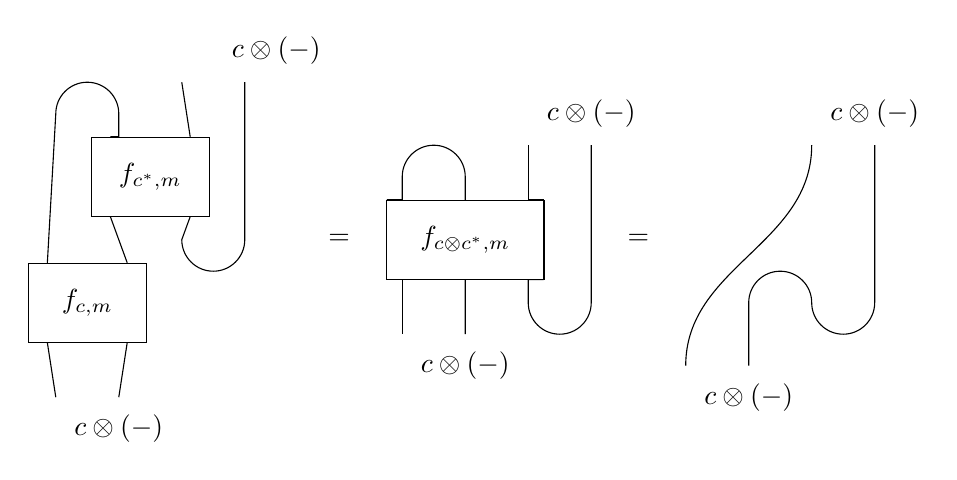
\begin{tikzpicture}[yscale=0.8, xscale=0.8, smooth]
	\node (A) at (2,2) [minimum height=1cm,minimum width=1.5cm, draw] {$f_{c^*,m}$};
	\node (B) at (1,0) [minimum height=1cm,minimum width=1.5cm, draw] {$f_{c,m}$};
	\draw (B.135) -- (.5,3) arc (180:0:0.5cm) |- (A.135) ;
	\draw (A.225) -- (B.45);
	\draw (A.45) -- (2.5,3.5);
	\draw (A.315) -- (2.5,1) arc (180:360:0.5cm) -- (3.5,3.5);
	\draw (B.315) -- (1.5, -1.5);
	\draw (B.225) -- (.5, -1.5);
	\node at (2.5,4) {$\cF$};
	\node at (4,4) {$c \otimes (-)$};
	\node at (.5, -2) {$\cF$};
	\node at (1.5, -2) {$c \otimes (-)$};
	
	\node at (5, 1) {$=$};
	
	\begin{scope}[xshift=5cm, yshift = -1cm]
		\node (A) at (2,2) [minimum height=1cm,minimum width=2cm, draw] {$f_{c \otimes c^*,m}$};
		\draw (A.153) -| (1,3) arc (180:0:0.5cm) -- (A.90) ;
		\draw (A.27) -| (3,3.5);
		\draw (A.333) -| (3,1) arc (180:360:0.5cm) -- (4, 3.5);
		\draw (A. 270) -- (2,.5);
		%\draw (A) -- (1,.5);
		\draw (A.207) -| (1,.5);
		\node at (3,4) {$\cF$};
		\node at (4,4) {$c \otimes (-)$};
		\node at (1,0) {$\cF$};
		\node at (2,0) {$c \otimes (-)$};
	\end{scope}
	
	\node at (9.75, 1) {$=$};
	
	\begin{scope}[xshift=10.5cm, yshift=-1cm]
		\draw (0, 0) to [out=90, in=270] (2,3.5);
		\draw (1,0) -- (1,1) arc (180:0:.5cm) arc (180:360:.5cm) -- (3,3.5);
		\node at (2,4) {$\cF$};
		\node at (3,4) {$c \otimes (-)$};
		\node at (0,-.5) {$\cF$};
		\node at (1,-.5) {$c \otimes (-)$};
	\end{scope}
\end{tikzpicture}
\end{center}
\end{proof}

The following Lemma was left as an exercise to the reader in \cite[\S 3.3]{EO-ftc}.

\begin{lemma} \label{lma:module-adjoint}
Let $\cC$ and $\cD$ be tensor categories. Let  $\cM$ and  $\cN$  be finite $\cC$-$\cD$-bimodule categories and let $\cF: \cM \to \cN$ be a $\cC$-$\cD$-bimodule functor.  If the underlying functor of $\cF$ has a right (respectively left) adjoint as a functor, then $\cF$ has a right (resp. left) adjoint $\cC$-$\cD$-bimodule functor. 
\end{lemma} \CD{This is a comment in EO, left to the reader, search for "observe that an adjoint to a module functor has a natural structure of the module functor"}
\begin{proof}
Suppose that $\cG$ is the right adjoint to the underlying functor of $\cF$, we will show that $\cG$ naturally has the structure of a $\cC$-$\cD$-bimodule functor.  The result for left adjoints is similar.

The binatural transformation $\psi_{x,n}: x \otimes \cG(n) \rightarrow \cG(x \otimes n)$ is given by the mate:
$$x \otimes \cG(n) \rightarrow \cG \cF(x \otimes \cG(n)) \rightarrow \cG(x \otimes \cF\cG(n)) \rightarrow \cG(x \otimes n)$$
where the first map is the unit of the adjunction, the second map is the binatural transformation coming from the module functor structure on $\cF$ and the third map is the counit.  
\CSP{This looks wrong to me. It doesn't seem to match the formula. Maybe it rotates the same way as the previous one?}
\NS{I think it's fixed now.  In some sense it rotates in the opposite direction as the previous argument, but we ended up doing the lax case for one and the oplax case for the other so they're the same.  Maybe that's misleading and we should change one of them.}
\begin{center}
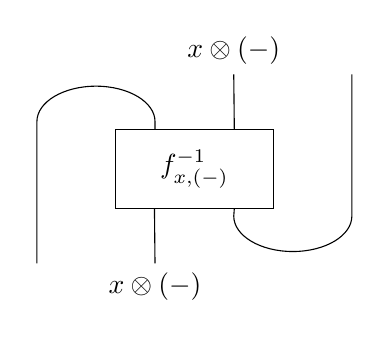
\begin{tikzpicture}[yscale=0.6]
	\node (A) at (2,2) [minimum height=1cm,minimum width=2cm, draw] {$f^{-1}_{x,\cG(-)}$};
	\draw (0,0) -- (0,3) arc (180:0:0.75cm) |- (A.135);
	\draw (A.225) -- (1.5,0);
	\draw (A.45) -- (2.5,4);
	\draw (A.315) -- (2.5,1) arc (180:360:0.75cm) -- (4,4);
	\node at (2.5,4.5) {$x \otimes (-)$};
	\node at (4,4.5) {$\cG$};
	\node at (0,-0.5) {$\cG$};
	\node at (1.5, -0.5) {$x \otimes (-)$};
\end{tikzpicture}
\end{center}

Applying the previous lemma, rigidity of $\cC$ and $\cD$ guarantees that this binatural transformation is an isomorphism.  The compatibility condition is left as an exercise.
\end{proof}

\begin{remark}
If $\cC$ and $\cD$ are not rigid, the argument in the proof of this lemma only shows that the right adjoint to an (oplax) module functor has a lax module functor structure, while the left adjoint of a (lax) module functor only has an oplax module functor structure.  %This is a serious issue as the following example shows. 
\end{remark}

\begin{lemma}\label{lem:partially_exact_action}
	Let $\cC$ be a tensor category and $\cM$ a $\cC$-module category. Then for each object $c \in \cC$, the action map $c \otimes (-): \cM \to \cM$ is exact. 
\end{lemma}
\CSP{I added this trivial lemma, it is probably in EGNO somewhere...}

\begin{proof}
	For each $c \in \cC$, the functor $c \otimes (-)$ admits both left and right adjoints, given by $c^* \otimes (-)$ and ${}^*c \otimes (-)$ respectively. 
\end{proof}



\subsection{Module categories are categories of modules}


Just as any finite linear category is a category of modules over an algebra, any finite module category over a finite tensor category is a category of module objects over an algebra object, as in Example \ref{ex:ModulesAreModules}.  This is one of the main theorems of \cite{EGNO}, and is essential to the structure theory of finite tensor categories.  The key construction underlying their proof is Ostrik's notion of the enriched hom for module categories \cite{MR1976459}.  

The following is an elaboration of results of \cite{MR1976459} and \cite{EO-ftc}. % Really: enriched is due to EOFTC sec 3.2 (Ost03 did the semisimple case), the rest is new.
\begin{proposition} \label{thm:enrichment-of-mod-cats}
	Let $\cC$ be a finite linear monoidal category and let $\cM$ be a finite $\cC$-module category. Assume that the action map $\cC \times \cM \to \cM$ is right exact in each variable. 
		Then $\cM$ is enriched, tensored, and cotensored over $\cC$ with the tensor structure coming from its structure as a $\cC$-module category. \CSP{added the right exactness condition.}
\end{proposition}

\begin{proof}
	What this means is that there exist functorial assignments of objects $\IHom(m', m) \in \cC$ and $(m^c) \in \cM$ for every $m,m' \in \cM$ and $c \in \cC$ and natural isomorphisms
	\begin{equation*}
		\Hom_\cC(c, \IHom(m', m)) \cong \Hom_\cM(c \otimes m', m) \cong \Hom_\cM( m', (m^c))
	\end{equation*}
	witnessing adjunctions
	\begin{equation*}
			c \otimes (-) \quad \dashv\quad (-^c) \quad \textrm{ and } \quad (-) \otimes m' \quad \dashv \quad \IHom(m', -).
	\end{equation*}
Such structure exists precisely if the functors
\begin{align*}
	\Hom_\cM((-)\otimes m', m): \; & \cC^\op \to \Vect \\
	\Hom_\cM(c \otimes (-), m): \; & \cM^\op \to \Vect
\end{align*}
are representable. In this case they represent the objects $\IHom(m', m)$ and $(m^c)$, respectively. Both of these functors are left exact, and hence by Corollary \ref{cor:representable} (which uses the finiteness of $\cC$ and $\cM$) both of these functors are indeed representable.  %\NS{I fixed a broken reference here, hopefully I got the right one.}
\end{proof}

\begin{remark}
	The existence of $\IHom(m', m)$ only requires $\cC$ to be finite and the action to be right exact in $\cC$, and similarly the existence of $(m^c)$ only requires $\cM$ to be finite and the action to be right exact in $\cM$.
\end{remark}

\begin{example}
Consider $\Vec$ as a module category over $\Vec(G)$.  Then $\IHom(1,1)$ is $k[G]$ with each $g$ put in grade $g$.
\end{example}



The goal of this subsection is to prove a generalization of the following result.

\begin{theorem}{\cite[Thm 2.11.6]{EGNO}, \cite[Thm 1]{MR1976459}} \label{thm:EGNO2.11.6}
	Let $\cM$ be a left module category over a finite tensor category $\cC$, and assume the action is right exact in $\cC$. If $\cM$ is finite as a linear category, then there exists an algebra object $A \in \cC$ together with an equivalence $\cM \simeq \Mod{}{A} (\cC)$ as left $\cC$-module categories. \CSP{added right exactness of the action in the C-variable}
\end{theorem}

\begin{example}
$\Vec$ as a $\Vec(G)$-module category can be realized as the category of modules over the group algebra $k[G] $ thought of as an object of $\Vec(G)$ by putting $g$ in grade $g$.  
\end{example}

Without assuming that the category $\cC$ is rigid this statement is false as the following example shows: 

\begin{example} \label{ex:lax-module}
	Let $\cR \cong \Vect \oplus \Vect \cdot X$ be the non-rigid linear monoidal category consisting of pairs of vector spaces, which we write as $V_1 + V_2 X$, with tensor product given by 
	\begin{equation*}
		(V_1 + V_2 X) \otimes (W_1 + W_2 X) = V_1 \otimes W_1  +  (V_1 \otimes W_2 \oplus V_2 \otimes W_1)X.
	\end{equation*} 
	Up to equivalence there are unique choices of associator and unitors making this a linear monoidal category. 
It is both finite and semisimple, and is a categorification of the ring $k[x]/(x^2)$, but it is not rigid. The object $X$ cannot have a dual as there is no object $Z \in \cR$ such that $Z \otimes X$ has a non-zero map to or from the unit object of $\cR$. 
	
	There is a tensor functor $F:\cR \to \Vect$ given by $(V_1 + V_2 X) \mapsto V_1$. This gives the category $\Vect$ the structure of a (left) $\cR$-module category, and moreover $F$ is naturally an $\cR$-module map. $F$ has both left and right adjoints, which agree and are given by the functor $G: \Vect \to \cR$ sending $W \in \Vect$ to $(W + 0 X) \in \cR$. It is not possible to give $G$ the structure of a (strong) $\cR$-module functor (c.f. Lemma~\ref{lem:laxisstrong}). Moreover there is no algebra object $A \in \cR$ such that $\Vect$ is equivalent to $\Mod{}{A}(\cR)$ as linear categories, let alone as $\cR$-module categories. 
\end{example}

In order to show exactly how rigidity appears we first prove a more general result which does not assume rigidity.  Stating this more general theorem requires the following definition.

\begin{definition}
	Let $\cC$ be a finite linear monoidal category and let $\cM$ be a finite $\cC$-module category. Assume that the action is right exact in $\cC$ so that $\cM$ is enriched over $\cC$. 
	An object $p \in \cM$ will be called {\em $\cC$-projective} if $\IHom(p, -)$ is right exact (it is automatically left exact). An object $p$ will be called a {\em $\cC$-generator} if $\IHom(p,-)$ is faithful.
	\CSP{added right exactness in C variable} 
\end{definition}

\begin{remark}
	An object $p \in \cM$ is a $\cC$-generator if and only if for each object $x \in \cM$ there exists an object $c \in \cC$ and a surjection $c \otimes p \twoheadrightarrow x$ if and only if for each object $x \in \cM$ the canonical map $\IHom(p,x) \otimes p \twoheadrightarrow x$ is a surjection. In particular an ordinary generator (i.e. an object such that $\Hom_\cM(p,-)$ is faithful) is also a $\cC$-generator. 
\end{remark}

\begin{example} \label{ex:rigid_all_C-proj}
	Let $\cC$ be a finite tensor category. We may view $\cC$ as a left $\cC$-module category over itself. Since $\cC$ is rigid, we have isomorphisms $\IHom(x,y) \cong y \otimes x^*$ and $(y^x) \cong {}^*x \otimes y$. Moreover Lemma \ref{lma:RigidIsExact} states that in this case the tensor product is exact in each variable, hence {\em every object} of $\cC$ is $\cC$-projective, even if the object is not a projective object in the usual sense. %\NS{To use that lemma you need to assume rigidity.}
\end{example}

Now we state the more general version of Theorem \ref{thm:EGNO2.11.6}.
%The following is an extension of \cite[Thm 2.11.2]{EGNO} and \cite[Thm 1]{MR1976459}.

\begin{theorem} \label{thm:C-module-Embedding} %!% [Thm 2.11.6(i)] 
	Let $\cM$ be a finite left module category over a finite, but not necessarily rigid, linear monoidal category $\cC$. Assume that the action is right exact in $\cC$. 
\CSP{added right exactness of action in C}
	Fix an object $p \in \cM$, and set $A = \IHom(p,p) \in \cC$. The object $A$ is naturally an algebra object in $\cC$, and gives rise to $\cC$-module functor:
	\begin{align*}
		F:   \Mod{}{A}(\cC) \to \cM \\
		F(x_A) := \coeq \left( x \otimes \IHom(p,p) \otimes p \rightrightarrows x \otimes p \right).
	\end{align*}
The functor $\IHom(p,-): \cM \to \Mod{}{A}(\cC)$ is right adjoint to $F$. 

Assume that $\IHom(p,-)$ may be equipped with the structure of a $\cC$-module functor and that the unit and counit of the adjunction $F \dashv \IHom(p,-)$ are morphisms of $\cC$-module functors. Assume further that $p$ is a $\cC$-projective $\cC$-generator.  Then the $\cC$-module adjunction  $F \dashv \IHom(p,-)$
	induces an equivalence of left $\cC$-module categories $\cM \simeq \Mod{}{A}(\cC)$. 
\end{theorem}

\noindent The proofs given in \cite{EGNO} and \cite{MR1976459} at first appear to depend on  the rigidity of $\cC$. Indeed the first step of the proof of \cite[Thm 2.11.2]{EGNO} invokes \cite[lemma 2.10.4.(4)]{EGNO} whose proof makes explicit use of rigidity. The same lemma is used in step (3) of the proof of \cite[Thm 1]{MR1976459}. However with a little care this is easily avoided (cf. \cite[Rmk. 2.11.3]{EGNO}). 

\begin{proof}[Proof of Thm.~\ref{thm:C-module-Embedding}]
	First, we have a series of natural isomorphisms:
	\begin{align*}
		\Hom_{\Mod{}{A}(\cC)}&(b, \IHom(p,x))  \cong \Hom_{\Mod{}{A}(\cC)}( \coeq \left( b \otimes A \otimes A_A \rightrightarrows b \otimes A_A  \right), \IHom(p,x)) \\
		& \cong \eq \left( \Hom_{\Mod{}{A}(\cC)}(b \otimes A_A, \IHom(p,x) )  \rightrightarrows \Hom_{\Mod{}{A}(\cC)}(  b \otimes A \otimes A_A, \IHom(p,x))  \right) \\
		& \cong \eq \left( \Hom_{\cC}(b, \IHom(p,x) )  \rightrightarrows \Hom_{\cC}(  b \otimes A, \IHom(p,x))  \right) \\
		& \cong \eq \left( \Hom_{\cM}(b \cdot p, x )  \rightrightarrows \Hom_{\cM}(  b \otimes A \cdot p, x)  \right) \\
		& \Hom_{\cM}( \coeq \left( b \otimes \IHom(p,p) \cdot p \rightrightarrows b \cdot p \right), x) \\
		& \Hom_{\cM}( F(b), x)
	\end{align*}
	where $b \in \Mod{}{A}(\cC)$ and $x \in \cM$. This establishes that $\IHom(p,-): \cM \to \Mod{}{A}(\cC)$ is indeed right adjoint to $F$.

For the second part of the theorem, our assumptions ensure that:
\begin{enumerate}
	\item the functor $\IHom(p, -)$ commutes (coherently) with the $\cC$-action;
	\item the functor $\IHom(p, -)$ is fully-faithful; and
	\item the functor $\IHom(p, -)$ is exact; 
\end{enumerate}
We wish to show that $\IHom(p, -)$ induces an equivalence of $\cC$-module categories. By Lemma \ref{lem:Recog_equiv_of_bimod} and (1), it is enough to show that it induces an equivalence of underlying categories. Moreover by (2) it is enough to show that the unit map $B \to \IHom(p, F(B))$ is an equivalence for all right $A$-modules $B$. This last statement follows from the following sequence of canonical isomorphisms (which utilize (2) and (3)):
\begin{align*}
	B & \cong \coeq \left( B \otimes \IHom(p,p) \otimes \IHom(p,p) \rightrightarrows B \otimes \IHom(p,p) \right)\\
	& \cong \coeq \left(\IHom(p,B  \otimes \IHom(p,p) \otimes p) \rightrightarrows \IHom(p,B \otimes p) \right)\\
	& \cong \IHom(p, F(B)). \qedhere
\end{align*}	
\end{proof}

%The Barr-Beck monadicity theorem\NS{Citation for Barr-Beck} implies that $\cM$ is equivalent to the category of algebras in $\cC$ for the monad $\IHom(p, (-) \otimes p)$. If the adjunction is $\cC$-linear, so in particular $\IHom(p,-)$ is a $\cC$-module functor, then this monad will be a ``$\cC$-module monad''. In this case the category of algebras for this monad is a $\cC$-module category and is easily identified with $\Mod{}{A}(\cC)$. \NS{Should this be written as an actual proof?}

If we additionally assume that $\cC$ is rigid, then some of the conditions of the previous theorem are automatically satisfied and become redundant. In particular Lemma \ref{lma:module-adjoint} and Lemma \ref{lma:Enough_C-projs} below imply that when $\cC$ is rigid the functor $\IHom(p,-)$ may always be enhanced to a $\cC$-module functor and moreover there always exists a $\cC$-projective $\cC$-generator.

\begin{lemma}{\cite[\S 2.11]{EGNO}} \label{lma:Enough_C-projs}
	If $\cC$ is a finite tensor category and $\cM$ is a finite module category, then there exists a $\cC$-projective $\cC$-generator. 
\end{lemma} \CD{This is point 1 after remark 2.11.3 in EGNO.} \NS{I added a reference}

\begin{proof}
	We claim that if $p \in \cM$ is a projective object (in the ordinary sense) then it is also $\cC$-projective. If this claim holds, then any (ordinary) projective generator of $\cM$ will be a $\cC$-projective $\cC$-generator, and these are guaranteed to exist since $\cM$ is finite. Thus assume that $p \in \cM$ is projective.  We aim to show that $\IHom(p, -)$ is right exact. 
	
	Since $\cC$ is a tensor category it is rigid, and hence we have a natural isomorphism of functors:
\begin{equation*}
	\Hom_{\cM}(c \otimes p, m) \cong \Hom_{\cM}(p, {}^*c \otimes m).
\end{equation*}
Taking an object to its dual is a (contravariant) equivalence of categories hence exact. Moreover since $p$ is projective and the $\cC$-module structure is right exact, we see that the above functor is left exact in the `$c$' variable and right exact in the `$m$' variable. Said differently, for each projective $p \in \cM$ we have a right exact functor
\begin{align*}
	G_p: & \; \cM \to \Fun^L(\cC^\op, \Vect) \\
	& m \mapsto (c \mapsto \Hom(c \otimes p, m)).
\end{align*}
By Theorem \ref{thm:enrichment-of-mod-cats} this functor factors through the Yoneda embedding as
\begin{equation*}
	\IHom(p, -): \cM \to \cC.
\end{equation*}
The claim now follows from the well-known fact that the Yoneda embedding reflects exact sequences. 
\end{proof}




\begin{proof}[Proof of Thm.~\ref{thm:EGNO2.11.6}]
By Lemmas \ref{lma:Enough_C-projs} and \ref{lma:module-adjoint}, the assumptions of Theorem~\ref{thm:C-module-Embedding} are satisfied.
\end{proof}

\begin{corollary} \label{cor:biexact_action}
	Let $\cC$ be a finite tensor category and let $\cM$ be a finite $\cC$-module category. If the action map $\cC \times \cM \to \cM$ is right exact in $\cC$, meaning that for each $m \in \cM$, $(-) \otimes m: \cC \to \cM$ is right exact, then the action is in fact exact in each variable separately (i.e. for each $c \in \cC$ and $m \in \cM$ the functors $c \otimes (-)$ and $(-) \otimes m$ are exact).  
\end{corollary}

\begin{proof}
	By Lemma~\ref{lem:partially_exact_action} the functor $c \otimes (-)$ is exact for each $c \in \cC$. We must show that $(-) \otimes m$ is exact for each $m \in \cM$. By Thm.~\ref{thm:EGNO2.11.6} there exists an algebra object $A \in \cC$, and an equivalence of $\cC$-module categories $\cM \simeq \Mod{}{A}(\cC)$. Hence there exists a forgetful functor $U:\cM \to \cC$ which is a $\cC$-module functor, is exact, and reflects short exact sequences. It follows that $(-) \otimes m: \cC \to \cM$ is exact if and only if $(-) \otimes U(m): \cC \to \cC$ is exact, but this follows from Lemma~\ref{lma:RigidIsExact}. 
\end{proof}

\begin{remark}
	By taking opposite categories, in the above corollary one may replace `right exact in $\cC$' with `left exact in $\cC$'. 
\end{remark}


\section{Construction of the relative Deligne tensor product} \label{sec:tc-deligne}

In this section we prove our main result, the existence of the Deligne tensor product of finite module categories over a finite tensor category.  We begin by recalling the definition of the Deligne tensor product from \cite{0909.3140}


\begin{definition}
	Let $\cC$ be a linear monoidal category. 
	Let $\cM$ be a right $\cC$-module category and $\cN$ a left $\cC$-module category. A {\em $\cC$-balanced functor} into a linear category $\cL$ is a right exact multilinear functor $\cM \times \cN \to \cL$ together with a natural isomorphism $\otimes^{\cM} \times id_{\cN} \cong id_{\cM} \times \otimes^{\cN}$ satisfying the evident pentagon identity. A {\em $\cC$-balanced transformation} is a natural transformation $\eta:F \to G$ of $\cC$-balanced functors such that the following diagram commutes for all $M \in \cM$, $C \in \cC$, and $N \in \cN$:
\begin{center}
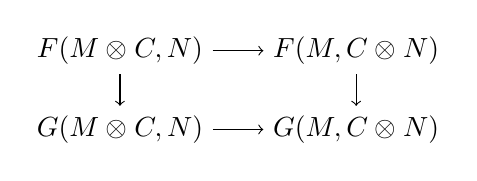
\begin{tikzpicture}
	\node (LT) at (0, 1) {$F(M \otimes^{\cM} C, N)$};
	\node (LB) at (0, 0) {$G(M \otimes^{\cM} C, N)$};
	\node (RT) at (3, 1) {$F(M, C \otimes^{\cN} N)$};
	\node (RB) at (3, 0) {$G(M, C \otimes^{\cN} N)$};
	\draw [->] (LT) -- node [left] {$$} (LB);
	\draw [->] (LT) -- node [above] {$$} (RT);
	\draw [->] (RT) -- node [right] {$$} (RB);
	\draw [->] (LB) -- node [below] {$$} (RB);
	%\node at (0.5, 1) {$\ulcorner$};
	%\node at (1.5, 0.5) {$\lrcorner$};
\end{tikzpicture}.
\end{center}
\end{definition}


\begin{definition}
	Let $\cM$ be a right $\cC$-module category and let $\cN$ be a left $\cC$-module category. The {\em relative Deligne tensor product $\cM \boxtimes_{\cC} \cN$} 
\CSP{Change this to `balanced tensor product'?}	
	is the universal linear category admitting a $\cC$-balanced right exact multilinear functor $\boxtimes_{\cC}: \cM \times \cN \to \cM \boxtimes_{\cC} \cN$. That is, there exists a $\cC$-balanced right exact multilinear functor $\boxtimes_{\cC}: \cM \times \cN \to \cM \boxtimes_{\cC} \cN$ which induces, for all linear categories $\cD$, an equivalence between the category of $\cC$-balanced right exact multilinear functors $\cM \times \cN \to \cD$ and the category of right exact linear functors $\cM \boxtimes_{\cC} \cN \to \cD$. 
\end{definition}

If it exists, the Deligne tensor product is unique up to equivalence, and this equivalence is in turn unique up to unique natural isomorphism. Said another way, the 2-category of linear categories representing the Deligne tensor product is either contractible or empty. 

In \cite{0909.3140} the existence of the relative Deligne tensor product was established for semisimple module categories over semisimple tensor categories over a field of characteristic zero.  A construction of the relative Deligne tensor product for finite tensor categories satisfying the additional assumption that $\cM \boxtimes \cN$ is exact as a $\cC$-bimodule category can be extracted from \cite[Thm 3.1]{1102.3411}. The following theorem extends these results to arbitrary finite tensor categories and finite module categories. 

\begin{theorem} \label{thm:DelignePrdtOverATCExists}
	Let $\cC$ be a finite tensor category and let $\cM_{\cC}$ and ${}_{\cC}\cN$ be finite right and left $\cC$-module categories, respectively. Then,
	\begin{enumerate}
		\item The relative Deligne tensor product $\cM \boxtimes_{\cC} \cN$ exists and is a finite linear category;
		\item If $\cM = \Mod{A}{}(\cC)$ and $\cN = \Mod{}{B}(\cC)$, then $\cM \boxtimes_{\cC} \cN \simeq \Mod{A }{B}(\cC)$;

		\item The functor $\boxtimes_{\cC}$ is exact in each variable and satisfies 
		\begin{equation*}
			\Hom_{\cM}(x,x') \otimes \Hom_{\cN}(y, y') \cong \Hom_{\cM \boxtimes_{\cC} \cN} (x \boxtimes_{\cC} y, x' \boxtimes_{\cC} y'),
		\end{equation*}
		\item Let $F_0: M \to M'$ be a right $\cC$-module functor and let $F_1: N \to N'$ be a left $\cC$-module functor. These induce a $\cC$-balanced functor $F: M \times N \to M' \times N' \to M' \boxtimes_{\cC} N'$. If $F_0$ and $F_1$ are exact, then so is the induced functor $\overline{F}: M \boxtimes_{\cC} N \to M' \boxtimes_{\cC} N'$.
		%If $F: \cM \times \cN \to \cD$ is a $\cC$-balanced multilinear functor which is exact in each variable, then it defines an exact functor $\overline{F}: \cM \boxtimes_{\cC} \cN \to \cD$. 
	\end{enumerate} 
\nid Here $\Mod{A}{B}(\cC)$ denotes the category of $A$-$B$-bimodule objects in $\cC$.
\CD{Add biexactness condition to Part (4) --- see email thread ``Deligne tensor product of rigids is rigid" and DTC.}
\CSP{I corrected part (4) and gave a proof.}	
\end{theorem}


\CD{Other new material (somewhere) as a result of the new issues? --- eg $Z(C)$ semisimple implies $C$ simple, etc.}

\begin{proof}
	 By Theorem \ref{thm:EGNO2.11.6}, there exist algebra objects $A, B \in \cC$ and equivalences $\cM \simeq \Mod{A}{}(\cC)$ and $\cN \simeq \Mod{}{B}(\cC)$. By Lemma \ref{lma:RigidIsExact}, the natural tensor product functor
	\begin{equation*}
		\cM \times \cN \simeq \Mod{A}{}(\cC) \times  \Mod{}{B}(\cC) \to \Mod{A}{B}(\cC)
	\end{equation*}
	is exact in each variable separately. It is also $\cC$-balanced. Thus $(2)$ implies both  $(1)$ and $(3)$. We will first prove (2), and then establish (4).  We wish to show that for any $\cD$ the category of right exact functors 
\begin{equation*}
	\overline{F}:\Mod{A}{B}(\cC) \to \cD
\end{equation*}
	is naturally equivalent to the category of $\cC$-balanced functors $F:\cM \times \cN \to \cD$ which are right exact in each variable separately. It is clear that every functor of the former type restricts to one of the later type, and so we must show that a functor of the later types extends uniquely (up to canonical isomorphism) to one of the former type. 
	
The key insight is to note that every object of $X \in \Mod{A}{B}(\cC)$ may be functorially written as a coequalizer of objects in the image of $\cM \times \cN$. For example we have:
\begin{equation*}
	{}_A A \otimes A \otimes X_B \rightrightarrows {}_A A \otimes X_B \to {}_A X_B.
\end{equation*}
Let $\delta: {}_A A \otimes A \otimes X_B \to {}_A A \otimes X_B$ be the difference map. 
For any right exact functor $\overline{F}$, the value $\overline{F}({}_A X_B)$ is canonically determined as a cokernel:
\begin{equation*}
	\overline{F}({}_A X_B) = \coker \left( \overline{F}(\delta): \overline{F}({}_A A \otimes A \otimes X_B) \to \overline{F}({}_A A \otimes X_B) \right).
\end{equation*} 
Moverover the modules ${}_A A \otimes A \otimes X_B$ and ${}_A A \otimes X_B$ are in the image of $\cM \times \cN$. 
	
Suppose we are given a $\cC$-balanced functor $F:\cM \times \cN \to \cD$ which is right exact in each variable separately. It is tempting to try to define the extension $\overline{F}: \Mod{A}{B}(\cC) \to \cD$ via a formula of the type:
\begin{equation*}
	\overline{F}({}_A X_B) := \coker \left( \underbrace{{F}(\delta)}_{\textrm{what is this?}}: F({}_A A \otimes A,  X_B) \to {F}({}_A A , X_B) \right).
\end{equation*} 
If this were possible, then it would immediately follow that the extension $\overline{F}$ is determined (up to unique natural isomorphism) by its restriction to $\cM \times \cN$, and that, moreover, the category of $\cC$-balanced exact-in-each-variable functors $F:\cM \times \cN \to \cD$ is equivalent to the category of functors  
$\overline{F}: \Mod{A}{B}(\cC) \to \cD$.

However it is not possible to define $\overline{F}$ in this way, at least not immediately. The difficulty is that while the relevant objects are in the image of $\cM \times \cN$, the map $\delta$ is not. 
Yet for each $X \in \Mod{A}{B}(\cC)$ we may form the following commutative diagram\footnote{The fact that this diagram commutes uses the coherence and naturality of the $\cC$-balanced structure. To verify the commutativity it is easiest to break each difference map into its constituent piece (one from the multiplication in either $A$ or $B$, and one from the action on $X$) and to show commutativity with respect to these maps.} 
%shown in Figure %\ref{fig:RelDelingePdtDiagram}.
%\begin{figure}[htbp]
	\begin{center}
		\begin{tikzpicture} \matrix (m) [matrix of math nodes, row sep={1.5cm,between origins}] {
		 F({}_AA \otimes A \otimes X, B \otimes B_B) &[1cm] F({}_AA \otimes X, B \otimes B_B) &[1cm] F({}_A X, B \otimes B_B) &[0.5cm] 0 \\
		F({}_AA \otimes A, X \otimes B \otimes B_B) & F({}_AA, X \otimes B \otimes B_B) & & \\
		F({}_AA \otimes A, X \otimes B_B) & F({}_AA , X \otimes B_B) & & \\
		 F({}_AA \otimes A \otimes X, B_B) & F({}_AA \otimes X, B_B) & F({}_AX,B_B)  & 0 \\
		& &\overline{F}({}_AX_B)  & \\
			};
			\draw [->] (m-1-1) -- node [above] {$\delta_1$} (m-1-2);
			\draw [->] (m-1-2) -- node [above] {$$} (m-1-3);
			\draw [->] (m-1-3) -- node [above] {$$} (m-1-4);
			\draw [->] (m-4-1) -- node [above] {$\delta_1$} (m-4-2);
			\draw [->] (m-4-2) -- node [above] {$$} (m-4-3);
			\draw [->] (m-4-3) -- node [above] {$$} (m-4-4);
			\draw [->] (m-1-1) -- node [left] {$\cong$} (m-2-1);
			\draw [->] (m-1-2) -- node [left] {$\cong$} (m-2-2);
			\draw [->] (m-3-1) -- node [left] {$\cong$} (m-4-1);
			\draw [->] (m-3-2) -- node [left] {$\cong$} (m-4-2);
			\draw [->] (m-2-1) -- node [left] {$\delta_2$} (m-3-1);
			\draw [->] (m-2-2) -- node [left] {$\delta_2$} (m-3-2);
			\draw [->,dashed] (m-1-3) -- node [left] {$\overline{\delta}_X$} (m-4-3);
			\draw [->,dashed] (m-4-3) -- node [left] {$$} (m-5-3);
			\node [node distance = 1.75cm, left of= m-5-3] {$\coker(\overline{\delta}_X)=:$};
		\end{tikzpicture}
	\end{center}
%	\caption{A digram useful for demonstrating the existence of the relative Deligne tensor product.}
%	\label{fig:RelDelingePdtDiagram}
%\end{figure}
Here the arrows labeled with isomorphisms come from the $\cC$-balanced structure of the functor $F$, while the remaining solid arrows are maps in the image of $\cM \times \cN$. The maps labeled with either $\delta_1$ or $\delta_2$ represent difference maps, as above. 

The rows of this diagram are exact (since $F$ was assumed to be right exact in each variable) and hence this diagram defines a unique map $\overline{\delta}_X$, shown as the long dashed arrow in the diagram. This is precisely the missing map, and hence we may define the value of the extension $\overline{F}$ on the object ${}_AX_B$ as the cokernel of $\overline{\delta}_X$. We leave it to the reader to verify that this extension gives a well-defined right exact functor 
\begin{equation*}
	\overline{F}: \Mod{A}{B}(\cC) \to \cD,
\end{equation*} 
and implements the desired equivalence between such right exact functors and $\cC$-balanced exact-in-each-variable functors. Verifying that this construction is well defined makes use of the pentagon identity satisfied by $\cC$-balanced functors. This establishes (1), (2), and (3). 

We now prove the final property. By Theorem \ref{thm:EGNO2.11.6}, there exist algebra objects $A, B, A'$, and $C' \in \cC$ and equivalences $\cM \simeq \Mod{A}{}(\cC)$, $\cN \simeq \Mod{}{B}(\cC)$, $\cM' \simeq \Mod{A'}{}(\cC)$, $\cN \simeq \Mod{}{B'}(\cC)$. Since $F_0$ and $F_1$ are right exact, they are equivalent to tensoring with bimodules:
\begin{align*}
	F_0(-) &\cong {}_{A'}x \otimes_A (-); \\
	F_1(-) & \cong (-) \times_B x_{B'}.
\end{align*}
Since $F_0$ and $F_1$ are exact, we may call these modules {\em flat} over $A$, respectively $B$. We wish to show that the induced functor:
\begin{equation*}
	\overline{F}(-) = {}_{A'}x \otimes_A (-) \times_B y_{B'}: \Mod{A}{B}(\cC) \to \Mod{A'}{B'}(\cC)
\end{equation*}
is exact. Since the forgetful functor $U: \Mod{A'}{B'}(\cC) \to \cC$ is exact and reflects short exact sequences, it is enough to show that 
\begin{equation*}
	x \otimes_A (-) \times_B y: \Mod{A}{B}(\cC) \to \cC
\end{equation*}
is exact. Let $0 \to m \to m' \to m'' \to 0$ be a short exact sequence of $A$-$B$-bimodules. We will compute the above functor in two steps, by first tensoring with $x$, and then with $y$. After tensoring with $x$ on the left we obtain a sequence of right $B$-modules:
\begin{equation*}
	0 \to x \otimes_A m \to x \otimes_A m' \to x \otimes_A {m''} \to 0
\end{equation*}
Since $x$ is flat, this sequence is exact after forgetting the $B$-module structure. Hence it is also an exact sequence of $B$-modules. Thus, since $y$ is flat, we obtain an exact sequence
\begin{equation*}
		0 \to x \otimes_A m \otimes_B y \to x \otimes_A m'\otimes_B y \to x \otimes_A {m''}  \otimes_B y \to 0
\end{equation*}
	as desired. 



The final property, part (4), now follows from a routine diagram chase, which we also leave to the reader. 
\end{proof}

\begin{example}
$\Vec \otimes_{\Vec(G)} \Vec$ is the category of $k[G]$-mod-$k[G]$ bimodules in $\Vec(G)$. Any left $k[G]$ bimodule is free, so we can identify $k[G]$-mod with $\Vec$, and thus $k[G]$-mod-$k[G]$ can be identified with $\text{mod-}k[G] \cong \Rep(G)$.
\end{example}

\begin{remark}
	If ${}_{\cD}\cM_{\cC}$ and ${}_{\cC}\cN_{\cE}$ are bimodule categories, then the actions of $\cD$ and $\cE$ induce a $\cD$-$\cE$-bimodule category structure on $\cM \boxtimes_{\cC} \cN$. This bimodule category satisfies the analogous universal property for $\cC$-balanced bilinear bimodule functors.   \NS{Why is the second sentence here true?  I find it surprising, but maybe I just need to think about it more.} \CSP{I think you just need to think about it more. Think about the case for ordinary algebras.}
\end{remark}

\begin{remark}
The above theorem assumes that $\cC$ is a finite tensor category, that is a finite rigid linear monoidal category.  The non-relative Deligne tensor product can be defined substantially more generally \cite{1212.1545}, and we hope that the relative Deligne tensor product can also be defined more generally.
\end{remark}
\CD{Add comment on importance/essentialness of right exactness in the theorem?}



\begin{lemma}%\label{lem:}
	\CSPcomm{Stronger version of (4) when field is perfect and $\cC = \Vec$}
\end{lemma}

\begin{corollary}%\label{cor:}
	\CSPcomm{Deligne tensor product over perfect fields preserves rigidity.}
\end{corollary}

\begin{lemma}%\label{lem:}
	\CSPcomm{Deligne tensor product of $\cC$ and $\cD$-modules.}
\end{lemma}





\bibliographystyle{alpha}
\bibliography{dtcbib}
\end{document}
